%!TEX root = ../prelims_main.tex
% \documentclass[../prelims_main.tex]{subfiles}

% \begin{document}

\section{Introduction}
\begin{multicols}{2}

\subsection{Outline}

\begin{itemize}
	\item Language Games
	\begin{itemize}
		\item Category structure of phonemes
		\item family resemlances in cognitive lit - why is phonetic identification a family resemblance strucutre?
		\item general statement of geometry of perceptual spaces
		\item family resemblances that differ in many senses really are defined by contrast between them -- which sense lets me distinguish the objects in question? put another way, selecting or rotating axes depending on short-term acoustic statistics.
		\item update to idea of perceptual geometry to include contextual dependence and reweighting
		\item Primary object is to learn the axes -- rather than learning some prebuilt structure that `exists in the world', brain has to figure out what parts of the world are informative, which is necessarily in context
	\end{itemize}

	\item Learning to play
	\begin{itemize}
		\item Infant speech learning, statistical regularity, perceptual warping
		\item general statement about the normalization of redundancy and adaptation to statistical regularity as a fundamental part of the auditory system (or maybe a brief allusion to it and discuss in more detail in neurophys section)
		\item But perceptual systems don't find `totally optimal' solutions as might be predicted from simpler experiments... 
		\item Representativeness means that there will be contributions from all the feature axes, even when they're irrelevant in the particular context.
	\end{itemize}

	\item Neurophys
	\begin{itemize}
		\item 
	\end{itemize}

\end{itemize}


\subsection{Phonemes are Language Games}

\begin{leftbar}

"Consider for example the proceedings that we call "games". [...] For if you look at them you will not see something that is common to all, but similarities, relationships, and a whole series of them at that. [...] Are they all 'amusing'? Compare chess with noughts and crosses. Or is there always winning and losing, or competition between players? Think of patience. [...] Look at the parts played by skill and luck; and at the difference between skill in chess and skill in tennis. 

And the result of this examination is: we see a complicated network
of similarities overlapping and criss-crossing: sometimes overall similarities, sometimes similarities of detail. [...] And we extend our concept as in spinning a thread we twist fibre on fibre. And the strength of the thread does not reside in the fact that some one fibre runs through its whole length, but in the overlapping of many fibres."

\textit{-Wittgenstein, Philosophical Investigations: 66-67\cite{wittgensteinPhilosophicalInvestigations1968}}

\end{leftbar}

Cognitive reality is characterized by its discreteness: rather than a continuous undifferentiated gradient wash of sensation and cognition, we experience objects, concepts, and categories. Speech is a continuous, high-dimensional, high-variability acoustic signal, yet it is perceived as a small number of relatively-discrete phonemes\cite{holtSpeechPerceptionCategorization2010a}. The acoustic structure of phonemes is a sort of "Family Resemblance"\cite{wittgensteinPhilosophicalInvestigations1968} --- the truly extravagant variability of speech has thus far defied any simple, definite acoustic parameterization of its phonemes. Instead, individual utterances within a phonetic category vary along high numbers of feature-dimensions, none of which are necessary nor sufficient for a listener to identify it\cite{Lisker1977,Bailey1980}.

\draft{There are different types of category structure, and what typifies family resemblance structures is 1) multiply defined - category membership is assesed across many imperfect `features' none of which is necessary nor sufficient, 2) prototypicality - some instances are better `examples' of a category than others, category membership is not binary, 3) context dependent - which feature is important depends on the features present in the instance and the context in which it is being compared. \cite{roschFamilyResemblancesStudies1975}}

\subsection{A Very Simple Model...}

Category representation theories are intimately related (and occasionally literally isometric to \cite{Edelman1998}) to theories of the measurement of similarity, which is dominated by geometric models\cite{Tversky1977}. These models nearly universally presuppose that categories exist in a feature space such that there exist some number of features that describe each instance of an object to be categorized.

To begin perhaps purposely naively, we will formulate a very simple geometric model of perceptual categories:

Suppose that some sensory stimulus $\mathbf{s}$ was composed of some set of physical attributes $a_i$ in the $d$-dimensional "stimulus space" $\mathbf{S}$ capable of fully representing all stimuli for a given sensory modality (as opposed to a particular set of eg. parameterized stimuli)

\begin{equation}
\label{eqn:s}
\mathbf{s} = \{a_0, a_i, \dots a_d\ : a \in \mathbf{S}\}
\end{equation}

For example, a digital sound is fully defined by the amplitudes of the waveform at each of its samples, or an image is defined as the wavelength and intensity of light at each pixel.  Since $a_i$ are arbitrary, $\mathbf{S}$ can represent a set of static attributes, or a set of attributes through time.

The sensory stimulus $\mathbf{s}$ is processed into some percept $\mathbf{p}$ composed of perceptual attributes $b_i$ in the $e$-dimensional "perceptual space" $\mathbf{P}$

\begin{equation}
\label{eqn:p}
\mathbf{p} = \{b_0, b_i, \dots b_e\ : b \in \mathbf{P}\}
\end{equation}

such that some perceptual computation $M$ maps $\mathbf{S}$ to $\mathbf{P}$

\begin{equation}
\label{eqn:map}
M = f: \mathbf{S} \to \mathbf{P}
\end{equation} 

\begin{equation}
\label{eqn:pfroms}
\mathbf{p} = M(\mathbf{s})
\end{equation}

from which the objective of the observer is to infer the category $c_s$ given $\mathbf{s}$ 

\begin{equation}
\label{eqn:infer}
c_s = max( \{ p(c_i | \mathbf{p}) : c_i \in \mathbf{C} \})
\end{equation}

The form of the sensory-perceptual mapping $M$, the perceptual space $\mathbf{P}$ it constructs, and the inference of category identity $c_s$ it supports serve as a loom for a few threads of the speech perception problem scattered across a few disciplines and vocabularies.

\subsection{...and its history}

\idea{Make sure to refer back to the 3 properties of family resemblance categories and use that to structure this section!!!}

A prominent strain of phonetics research in the US, largely associated with the Haskins Labs (\cite{schertzPhoneticCueWeighting2020} and see \cite[p.~51]{ohalaGuideHistoryPhonetic1999}), has characterized the speech perception problem as resolving a set of acoustic "cues" into phonetic identity:

\begin{leftbar}
"Liberman, Cooper, and Pierre Delattre began to study the acoustic speech signal, to determine how it represents the consonants and vowels of spoken words, and to discover the acoustic structure (the `cues') essential for their identification by listeners. [\dots] By selectively including and eliminating elements of acoustic structure,l Liberman and his colleagues could determine what bits of structure provided information for the different phonetic properties of spoken words."

-Carol Fowler \& Katherine S. Harris in \cite[p.~51]{ohalaGuideHistoryPhonetic1999}
\end{leftbar}

The "cue discovery" paradigm of phonetics research posits that, for the auditory component of phonetic perception, the elements in $\mathbf{P}$ are linear combinations of the features in $\mathbf{S}$ whose manipulation can influence the identity of the perceived phoneme. These features represent familiar phonetic parameterizations like voice onset times or formant frequency ratios. The mapping $M$ that constructs $\mathbf{p}$ is taken to be a fixed, innate feature of the auditory system: "this version of the auditory theory takes the perceived boundary between one phonetic category and another to correspond to a naturally-occurring discontinuity in perception of the relevant acoustic continuum." \cite{Liberman1985a}. 

The conclusion of cue-based research is summarized neatly by Philip, Robert E. Remez, and Jennifer Pardo with respect to their sinewave synthesis experiments: "Question: Which acoustic elements are essential for the perception of speech? Answer: None\cite{HaskinsLaboratories2020}." The failure to find a simple parameterization of phonetic categories as acoustic cues motivated an abandonment of an acoustic account of phonetic perception entirely in favor of a motor theory of perception that positied a special, evolved "speech module" that linked the wily acoustics of speech sounds to the action of the articulatory system:

\begin{leftbar}
"For if phonetic categories were acoustic patterns, and if, accordingly, phonetic perception were properly auditory, one should be able to describe quite straightforwardly the acoustic basis for the phonetic category and its associated percept. According to the motor theory, by contrast, one would expect the acoustic signal to serve only as a source of information about the gestures; hence the gestures would properly define the category"
\cite{Liberman1985a}
\end{leftbar}

Purely motor theories of speech have been diversely problematized, not least of all by the many demonstrations that animals that conspicuously lack a human articulatory system are capable of phonetic categorization\cite{Carbonell2014,Lotto1997,Kluender2000}. The acoustic problem of speech perception was simply too difficult to be solved by an evolutionarily plausible auditory system -- how could the family resemblance structure of phonetic categories be learned without some explicit, innate knowledge of the acoustic consequences of articulation?\cite{Bailey1980} 

Research on infant acquisition of speech sounds has since demonstrated the profound plasticity of the auditory system and its ability to learn the complex statistical dependencies between the acoustic attributes of speech\cite{kuhlNewViewLanguage2000}. A family of models based primarily on the work of Patricia Kuhl and colleagues describe the stimulus space $\mathbf{S}$ as acoustic features based on the "basic cuts" of sensitivity in the auditory system\cite{kuhlEarlyLanguageAcquisition2004}. Infants exploit the statistical regularity and patterns of feature co-uccurance to learn some mapping $M$ that constructs a "warped" perceptual space $\mathbf{P}$ that clusters features in $\mathbf{S}$ into acoustic "prototypes."\cite{kuhlNewViewLanguage2000} 

Phonetic category identity then consists of some density in $\mathbf{P}$, the center of which is the "ideal" phonetic exemplar most likely to be identified with a particular categoery, and proceeding from this center point one transitions from off-target imperfect examplars to overlapping densities of other phonetic categories. Extensions to the model make this formulation explicit, like Kronrod, Coppess, and Feldman's\cite{Kronrod2016a} bayesian model that offers a unified explanation of the strong categorical perception of stop consonants and the weaker categorical perception of vowels. Their model describes phonetic identification as an inference problem that depends on both the acoustic properties of a stimulus and prior knowledge of phonetic categories, defined as some mean and variance in an arbitrary perceptual space. 

\draft{In this model, the difficulty of the acoustic problem of speech perception carefully described by cue-centric phonetic research is resolved by suggesting the auditory system relies on sharp internal representations of category identity for phonemes that have a large degree of uninformative variaance, like stop consonants.} 

\draft{The degree of arbitrariness is problematic for the model, however. The proposition that there is some stimulus space $\mathbf{P}$ that supports linearly-separable phonetic categories is emphatically counterevidenced by the 70 years of cue-based research that has attempted to find one (cite violations of gestalt principles from \cite{remezPerceptualOrganizationSpeech1994} and \cite{Lisker1977}). These prototype models, without weighting for the informativeness of a particular dimension in context (as opposed to some global weight) would be vulnerable to misidentifying speech when the most dominant cue was made redundant, when in fact human listeners will adapt to using a more informative cue. In fact a lot of the research relies on carefully parameterized speech, so if they considered the cases where those cues failed then such a single-density-based prototype model. Having nonlinear blobby parameterizations of prototypes doesn't really solve the problem either, as you would then just require an additional downstream `readout' layer that could compute the conditions where a particular dimension }


\draft{Their future directions says that identifying and learning the dimensions is of critical importance, we can extend our model by continuing Kronrod's emphasis on the information contained in each perceptual dimension and allow it to vary by context...}

\subsection{An extension to our model...}

Instead of a static perceptual space $\mathbf{P}$ where a given stimulus $\mathbf{s}$ is mapped to a single percept $\mathbf{p}$ (ie. $M$ is injective), we can extend our very simple model by introducing some notion of reweighting perceptual dimensions. Rather than inferring category directly from $\mathbf{P}$ as in eq. \ref{eqn:infer}, the features $b_e \in \mathbf{P}$ are reweighted by some weight vector $\mathbf{w}$ computed as some function $W$ of the representation $\mathbf{p} = M(\mathbf{s})$ and some prior knowledge of the category structure of $\mathbf{C}$

\begin{equation}
\label{eqn:w}
\mathbf{w} = W(\mathbf{p}, \mathbf{C})
\end{equation}

\begin{equation}
\label{eqn:infer_2}
c_s = max\big( \big\{ p(c_i | \mathbf{p} \cdot \mathbf{w}) : c_i \in \mathbf{C} \big\}\big)
\end{equation}

Recall that since the features $a \in \mathbf{S}$ are arbitrary, they can include time-varying features, so the weighting function $W$ can, for example, incorporate contextual effects from the recent perceptual past. Category inference being dependent on $W$ has equivalent interpretations in the parlance of artificial neural networks and geometry: as a self-attention mechanism (eg. \cite{vaswaniAttentionAllYou2017}) giving higher weight to more informative features, or as "collapsing" or "expanding" un/informative dimensions. 

\subsection{And its implications...}

The notion of different perceptual features having different weights or importance depending on the acoustic context and the category structure of the phonemes for a particular language is of course far from new. 

\todo{cue weighting, different types of cues, contextual and informative \cite{schertzPhoneticCueWeighting2020}}

A parallel line of thought to the generative models that posit phonetic identity as some positive description of cues or perceptual features are discriminative models that focuses on the features that can be used to tell phonemes apart. A prominent family of discriminative models in phonetics are those that describe a hierarchy of contrastive features\cite{Dresher2008,clementsFeatureOrganization2006,halleFeatureSpreadingRepresentation2000}. Though they are diverse in their details, in these models $M$ is again typically some fixed feature of the auditory system, and the perceptual space $\mathbf{P}$ that it constructs is some set of high-level descriptions like voicing, frication, or articulator configuration. Typically these features are binary (eg. +/- voiced), rather than continuous.

\begin{figure}[H]
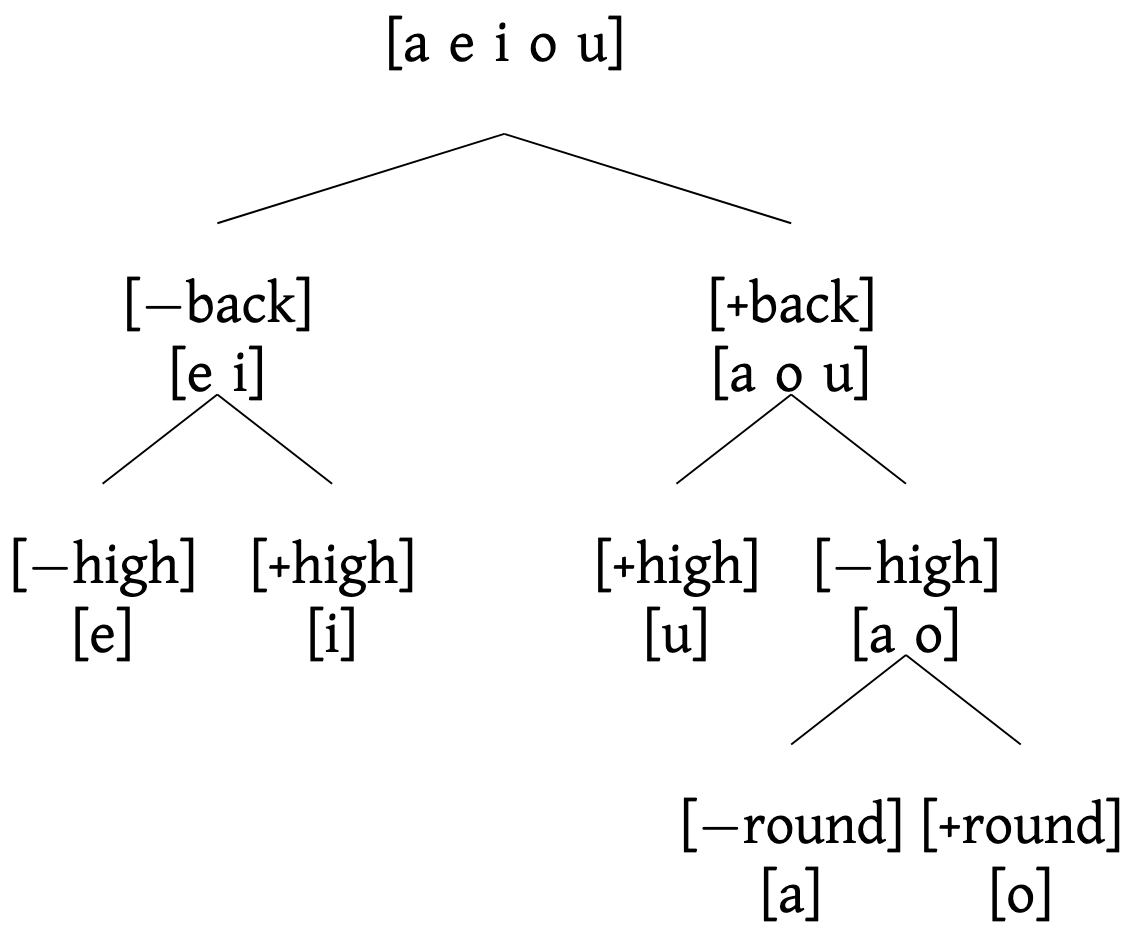
\includegraphics[width=\columnwidth]{russian_vowel_hierarchy.png}
\caption{Contrastive hierarchy for Russian Vowels, reproduced from \cite{iosadVowelReductionRussian2012} without permission}
\label{fig:hierarchy}
\end{figure}

As an example, consider the proposed contrastive feature hierarchy for russian vowels from \cite{iosadVowelReductionRussian2012} (Figure \ref{fig:hierarchy}). Vowel identification is dominated by the primary contrast of +/- back, and successive constrastive features eliminate candidate phonemes until the true phoneme is identified. $W$'s dependence on $\mathbf{C}$ is exemplified (\todo{fix passive voice..}) by its treatment of "round": -back vowels [e i] are fully determined by +/- high, so for a percept $\mathbf{p}$ with -back, the weight of "round" should be 0. Put another way, the importance of a given feature is dependent on the phonemes that are left ambiguous without it. Any given feature's importance depends on both the set of available features and the set of available categories. 

\todo{features like +rhotic though don't correspond to anything in the input space tho\cite{lindauStory1980}}

\draft{expand here on how parameterized stimuli with a single contrast aren't really modeling the problem: like shouldn't it matter how bad the speech sounds sound for claims about natural speech perception? the real question is, during perception, how are the different perceptual axes normalized/selected/weighted; during learning, how does the auditory system learn the space of features? When there is only one feature present the auditory system is performing a qualitatively different task. The use of parameterized stimuli is itself a strong assumption on the nature of the problem that the auditory system is solving. Even parameterizing a family resemblance is so because you assume the weight and salience of different cues. Additionally since there is some "basic cuts" argument to be made about the auditory system and the types of cues that it selects, you're unlikely to hit those if you just use some arbitrary array of stimuli: speech sounds come pre-optimized for mammalian auditory systems (though obvs mice aren't people) a la adaptive dispersion }

\draft{"I should emphasize, nevertheless, that there is a great deal of evidence that practice, even large amounts of it, does not produce efficient perception of acoustic alphabets. This is clear, not only in the example of the Morse code, but even more convincingly, perhaps, in the repeatedly unsuccessful attempts to find nonspeech sounds that will work well as part of a reading machine for the bling. Many sound alphabets have been given a thorough trial, but none has proved adequate. It must surely give us pause to know that, while sounds are the universal carriers of language, only one set of sounds --- those of speech --- serves well."\cite{libermanCharacteristicsPerceptionSpeech1970} Their conclusions are wrong -- that this means that speech is special and has its own processing modality -- but the observation does indeed point to the joint optimization of a phonetic space over an auditory space as being constitutive of language, and a potent reason to use speech sounds for category learning.}


The notion of the informativeness of different featural dimensions has been given its \draft{fullest} treatment in Keith Kluender and Christian Stilp's application of information theory to phonetic perception\cite{kluenderLongstandingProblemsSpeech2019a,kluenderPerceptionVowelSounds2013,stilpEfficientCodingStatistically2012,stilpRapidEfficientCoding2010}. They summarize their argument, elegantly as always:

\begin{leftbar}
"If one's problem is finding the right fencing to corral a unicorn, then there is really no problem at all. Instead the problem is dissolved upon discovery that unicorns do not exist.

Here, we ask the reader to consider the possibility that there are no objects of perception [...]. Like unicorns, they do not exist at all. Instead, there are \textit{objectives} for perception. [...] Perceptual success does not require recovery or representations of the world per se." \cite{kluenderLongstandingProblemsSpeech2019a}
\end{leftbar}

They argue that the central operation of sensory systems is to adapt to regularity at multiple scales in order to efficiently extract meaningful information from their environment. Rather than a faithful representation of articulatory maneuvers (as in motor theory) or a warped, but still bijective relationship between the acoustic space and perceptual space (as in perceptual warping), they argue that sensory systems discard information that is predictable based on (multiscale) context, and instead represent just the unpredictable, "information-bearing" in an appropriately Shannonistic sense, dimensions. 

Though theoretically all configurations of frequencies and amplitudes are possible, naturally produced sounds are strongly constrained by the physics of their production -- much of the variation in natural sounds is predictable. Rather than representing the fullness of acoustic variation, the auditory system adapts to redundancies and regularities in sounds to preferentially represent only the unpredictable, informative variation in an "efficient code" \cite{smithEfficientAuditoryCoding2006a,Geffen2011}. In the case of phonetic perception, where the objective of the listener is to identify the phoneme intended by the speaker rather than perceiving a sound qua sound, the listener attempts to learn auditory features that are maximally informative of phonetic identity\cite{kiefteAbsorptionReliableSpectral2008,liuOptimalFeaturesAuditory2019,kluenderLongstandingProblemsSpeech2019a,kluenderPerceptionVowelSounds2013}.

This information-theoretic account provides a mechanism for learning the dimensions of $\mathbf{P}$ and the form of $W$. Rather than some a priori, fixed inventory of articulatory/acoustic cues, a listener should learn some set of perceptual features that support the identification of phonemes given the phonemic inventory of their language and the acoustic variability (eg. accent, environment, timbre, etc.) that they are exposed to. Individual listeners do indeed use different combinations of cues with different weights\cite{iversonInfluencesPhoneticIdentification1996} which are stable over time\cite{souzaReliabilityRepeatabilitySpeech2018}. Rather than learning some category center and spread over some pre-existing perceptual feature space, the task of the listener is to learn the feature space itself. 

The difference between learning $\mathbf{P}$ and the operation of $W$ is a matter of timescale: over short timescales, $W$ reweights the features in $\mathbf{P}$ depending on those features that are contextually informative of phonetic identity. While the observation that individual cues are informative, uninformative, and anti-informative depending on the context of surrounding phonemes is a central feature of argument for a motor theory\cite{Bailey1980}, an information-theoretic view interprets this problem as a reweighting of individual features: /s/ differs from /f/ along different featural axes than /s/ differs from /k/, so /s/ shouldn't necessarily rely on the same inventory of acoustic features in all contexts. Contextual effects on phonetic categorization are of course well known (see \cite{holtSpeechPerceptionCategorization2010a}). Where perceptual warping accounts cannot explain results where some or all of the typical acoustic features are replaced, like sine-wave speech\cite{remezSpeechPerceptionTraditional1981}, noise-vocoded speech\cite{davisLexicalInformationDrives2005}, or joint spectrotemporal degradation\cite{elliottModulationTransferFunction2009a}; an information-theoretic view argues that listeners will adapt to use any cues that are still present (as in \cite{kiefteAbsorptionReliableSpectral2008}). 

The auditory system does \textit{not} seem to operate in an entirely information-maximizing way when identifying phonemes, however. Consider a category structure like that used by Couchman, Coutinho, and Smith (2010, \cite{couchmanRulesResemblanceTheir2010}) depicted in figure \ref{fig:rule_based}. Each stimulus is composed of four binary features (columns), and stimulus identity is defined by the first feature (0 = category A, 1 = category B). The remaining three features are "epiphenomenal," but stimuli in category B have a greater sum than those in category A. A perfect, information-maximizing observer would learn to only attend to the first dimension, but in speech and many other perceptual categories observers use many, even uninformative dimensions\cite{couchmanRulesResemblanceTheir2010,roschFamilyResemblancesStudies1975} (but see \cite{leaUseMultipleDimensions2008}). Non-speech sounds that are strictly uninformative of phonetic identity like pure tones and sweeps can nevertheless strongly influence the perceived phoneme\cite{holtNeighboringSpectralContent2000,holtMeanMattersEffects2006}, even when the sounds are not immediately adjacent\cite{holtTemporallyNonadjacentNonlinguistic2005}. Such an influence of many, imperfect stimulus dimensions on perception is our signpost to indicate we've arrived back in the bewildering little shire of category structures with family resemblance.

The differing (often implicit) assumptions about the \sarcasm{very complicated model™} characterize the major historical disputes in categorical phonetic perception, but also \draft{<suggest the kinds of experiments that might resolve them>.}

\todo{expand on each of these: a)} Arguably, the careful work of cue theorists led them to motor theories of perception because of a characterization of $M$ as fixed that made the non-invariant acoustic structure of phonetic categories impossible for the auditory system to compute. \draft{but their work was extremely valuable because it explicated the nonlinear nature of acoustic cues and the family resemblance structure of acoustic properties.} \todo{b)} Work in animal models and infant speech perception demonstrated that phonetic categories were indeed learned \todo{(cite infants can acquire all phonemes)}, but the use of parametric stimuli led to overly-parsimonious models that don't capture the true scope of the problem. \todo{need experiments that satisfy the "real problem" (review previous sections and highlight each of the ways the family resemblance structure of phonemes indicates a particular experimental design parameter, but that we need to finish it by adding a neural layer... which we get to in the next section...)}

\draft{Integrate this into the discussion about infant speech learning research in previous para - 
The idea that speech acquisition necessarily involves learning the features that are maximally informative is demonstrated by the ability for infants to discriminate between the phonemes of any language, but during language acquisition become specifically attuned to the phonemes of the language(s) they are taught. Though this is typically discussed as learning the statistical regularities of speech  sounds (\textcolor{red}{need to cite more because claim of typicality}\cite{kuhlPhoneticLearningPathway2008}\cite{kuhlEarlyLanguageAcquisition2004}), the act of emphasizing the statistical regularity must necessarily mean collapsing those phoentic contrasts that are not present in the language -- they aren't informative because no one uses that contrast. \draft{indeed they trade off -- infants that are better at discriminating the phonemes in their language are worse at discrmiinating those in a non-native language\cite{kuhlPhoneticLearningPathway2008}} (babies initially can learn all phonemes\cite{kuhlEarlyLanguageAcquisition2004}, so they have to learn some feature which necessarily compresses the auditory space\cite{ForeignlanguageExperienceInfancy})}

\draft{and focusing on the acquisition of informative stimulus dimensions fundamentally alters the research question. The problem is the mutual translation/misundertanding of what cues *are* -- a lot of neurophys research into language ends up using parameterized speech because we want to create parameters and then look for analogies in the brain, either in single neurons or populations. Neuroscientists interpret these cues as `constitutive' of the phoneme rather than a particular cue describing it (try to find ye old phonetics lit that talks about cue validity as being a problem even in phonetics). This is the pt to turn to `so instead we need to let the brain reveal its order to us, when presented with a complex array of stimuli, which features does the brain encode and how are they represented???'}

 \begin{figure}[H]
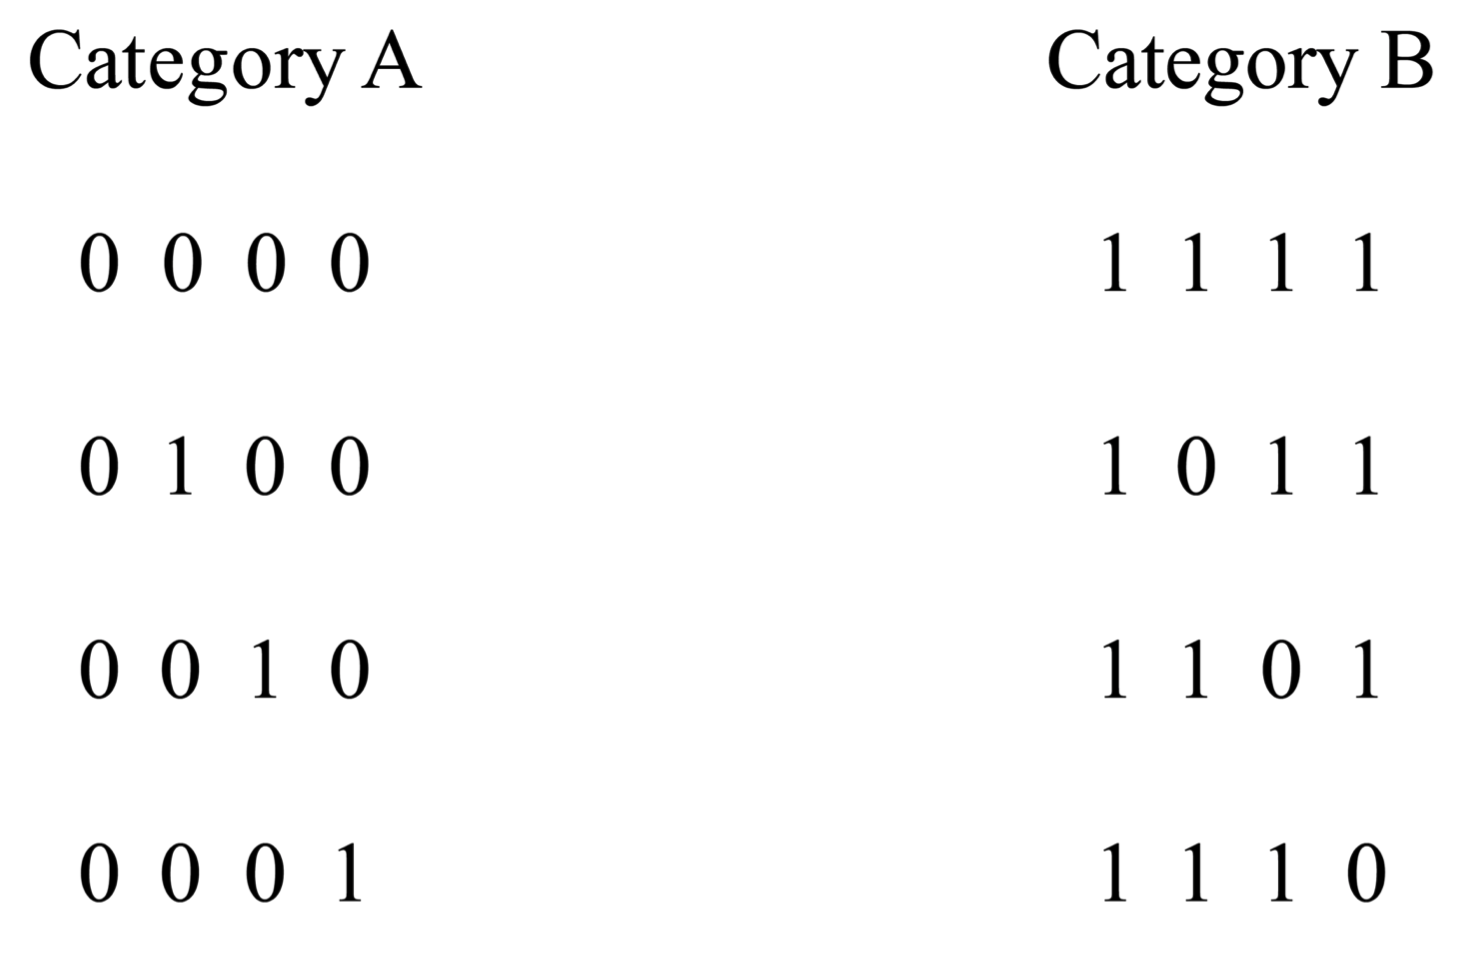
\includegraphics[width=\columnwidth]{rule_based_categorization.png}
\caption{Category structure reproduced from \cite{couchmanRulesResemblanceTheir2010} without permission. Each stimulus (row of four digits) is composed of four features (columns). Category identity is determined by the first feature (0 = A, 1 = B), but three other "irrelevant" features are present.}
\label{fig:rule_based}
\end{figure}




% \end{document}